Figure xxx sumarizes the general methodology that will be discussed. 


As a baseline we deploy a vanilla OpenDataCam setup using its built-in tools for object counting and path recording.
From the OpenDataCam GUI it's possible to visually inspect the detected objects and draw line counters 
which keep track of the total number of objects passing the line given a certain areal threshold and approach angle. 
The line counters are bi-directional and segment totals based on the mode of transportation.

\ \\
The baseline will focus on the capabilities of only applying OpenDataCam and its tools. This will mostly be "trafic shares" for 
different paths and directions. 
\\ 
We then go on with further data processing as an extension. The main goal is to have a tool catered to analyzing cyclists, capturing
discrete desire lines (with magnitude) and the ability to "hook into" video material for certain scenarios.

\subsection{Hardware}
The pipeline for our setup is shown below on figure \ref{system}. OpenDataCam uses the Yolo4 weights to localize cyclists and pedestrians.
Processing was executed on an ARM based NVIDIA Jetson Xavier NX (development board) equipped with a 384-core NVIDIA Volta GPU
and 8GB of memmory. 

\raggedbottom
\noindent
\begin{tabular}{@{}cc}
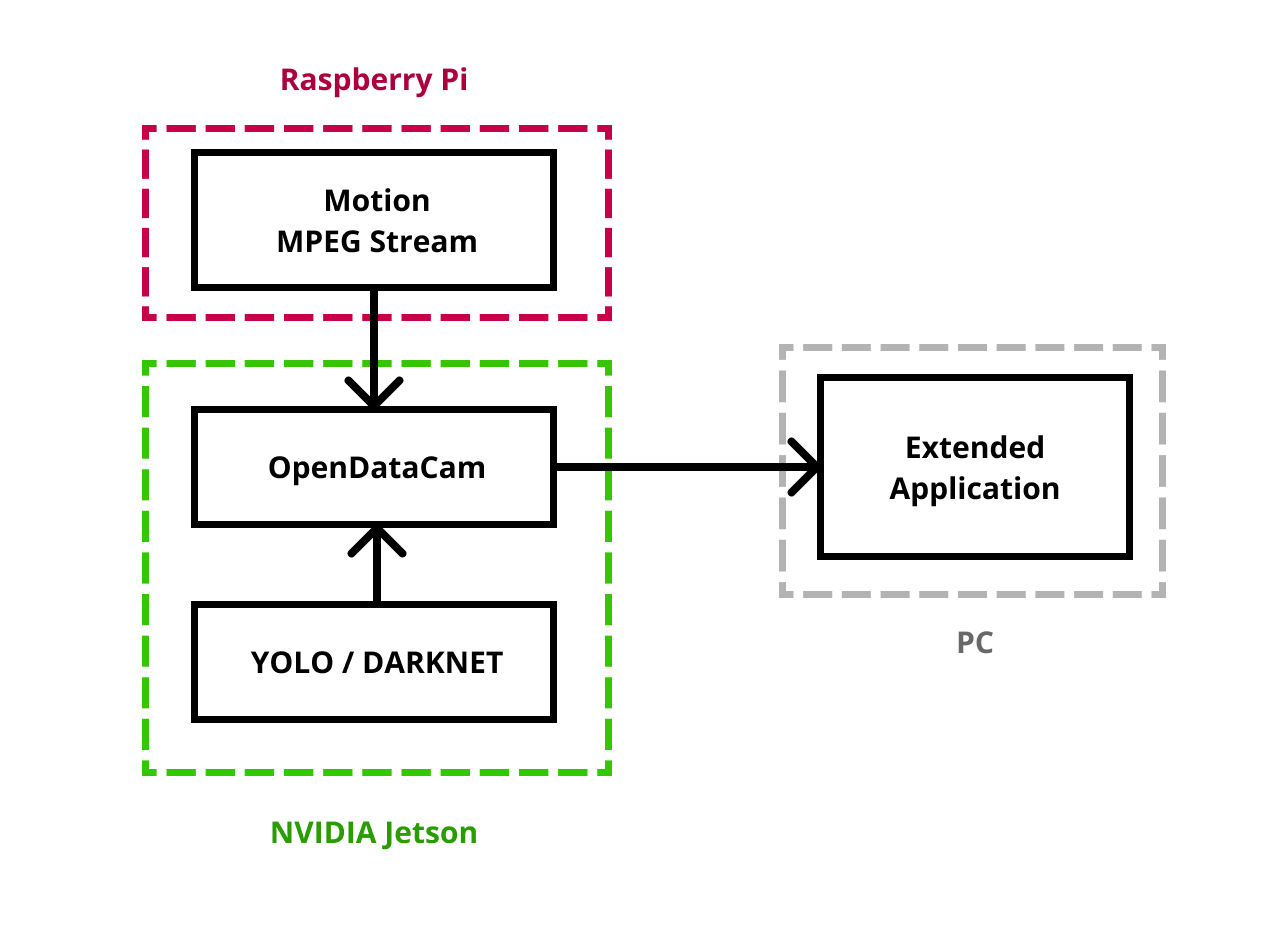
\includegraphics[width=1.0\columnwidth]{system} 
\end{tabular}
\captionof{figure}{System overview}
\label{system}

\ \\
The video feed for YOLO is provided through the OpenDataCam interface, which allows for real-time analysis through an onboard camera
or a video stream from an IP camera. 

\ \\
For further analysis the raw data from the recordings was exported in the form of CSV and JSON files. This includes both the low-level
object detection (bounding-boxes, frame reference, confidence levels etc.) and the totals from the line counters.

\subsection{Case study}
The Dybbølsbro intersection in Copenhagen was chosen as the location for our primary data collection. 
The Dybbølsbro intersection faces several traffic flow challenges as a result development in the immediate vicinity as well as being a large intersection.
These challenges make the Dybbølsbro intersection one of the more extreme in Copenhagen and would serve as a good base to this quantitative analysis method. 

To determine the desire paths that cyclist take throughout the Dybbelsbro intersection we recorded XX hours of footage 
at the Dybbølsbro intersection from X different camera angles.
The considerations taken in choosing a camera angle were:

\begin{itemize}
	\item Camera visibility to cyclists.
	\item Adequate mounting points, in terms of height and surface.
	\item Special attention was also given to making sure that cameras were not mounted on traffic signage.
\end{itemize}

\subsection{Trajectory projection}
The video footage was analyzed using OpenDataCam which is an abstraction layer on top of Yolo. Yolo being an object detection library for object detection in images.
Once the video is analyzed by OpenDataCam, we receive a .json file containing a Unique ID for each identified cyclist that is detected for each frame of the video file. 
The unique ID is accompanied by bounding box coordinates of the detected bicycle on the frame. 
The center-bottom coordinates of the bounding box over multiple frames represents the track of an identified bicycle.

\ \\
By assuming the road as a 2D plane, hereby ignoring any non-linear deformations (e.g. from lens distortion or curvature of the pavement), 
we can transform the pixel positions from the video to real-world 2D coordinates. 
We calculate the \textit{homography matrix}, describing the transformation from one plane to another, by mapping four reference points from each frame (figure \ref{projection_figure}).

\raggedbottom
\ \\ 
\noindent
\begin{tabular}{@{}cc}
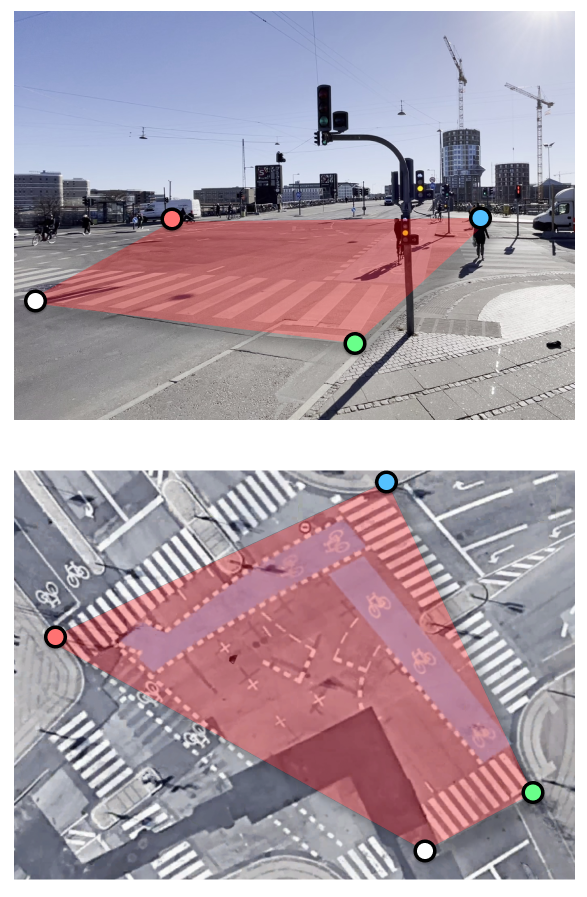
\includegraphics[width=1.0\columnwidth]{projection_figure} 
\end{tabular}
\captionof{figure}{Reference points on map projection}
\label{projection_figure}

\ \\
Figure \ref{pipeline} summarizes the general methodology that will be discussed. We will focus
on three main components, Data collection, Data processing and Data exploration.

\ \\ 
\noindent
\begin{tabular}{@{}cc}
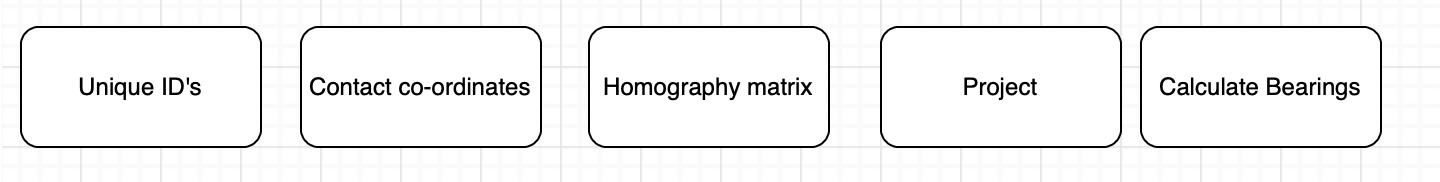
\includegraphics[width=1.0\columnwidth]{temp.png} 
\end{tabular}
\captionof{figure}{Data pipeline overview} 
\label{pipeline}

\subsection{Data Collection}

The Dybbølsbro intersection in Copenhagen was chosen as the location for our primary data collection. 
The Dybbølsbro intersection faces several traffic flow challenges as a result development in the immediate vicinity as well as being a large intersection.
These challenges make the Dybbølsbro intersection one of the more extreme in Copenhagen and would serve as a good base to this quantitative analysis method. 
As Dybbølsbro is a large intersection we use two cameras on opposite side of the intersection in order to get a good overview of the intersection regardless of the traffic obstructing views.

\subsection{Recording Location}

There are three consideration to take into account when applying these methods to an intersection.
\begin{itemize}
	\item1. Intersection size.
	\item2. Camera mounting points.
	\item3. Intersection composition
\end{itemize}

\subsection{Camera Selection}

Modern mobile phones offer high resolution and quality cameras in a compact design. We used an LG G6 and a Samsung S7 Edge for recording the intersection.
These devices offer wide enough field-of-views (FOV) to record the parts of the intersection we are interested in from the selected mounting locations.
FOV being the maximum area a camera can image. A formal method of selecting a recording device would be to select one that has a large enough FOV that can image the entire intersection 
from the mounting position that is closes to the intersection. Given a recording location we can calculate the FOV needed using equation \ref{eq:1}.
If $\theta > FOV$ then the FOV is too small.
\begin{equation}
    \theta = tan^-1(\frac{\frac{width}{2}}{adjacent}) * 2\label{eq:1}
  \end{equation}

\ \\ 
  \begin{figure}[h]
    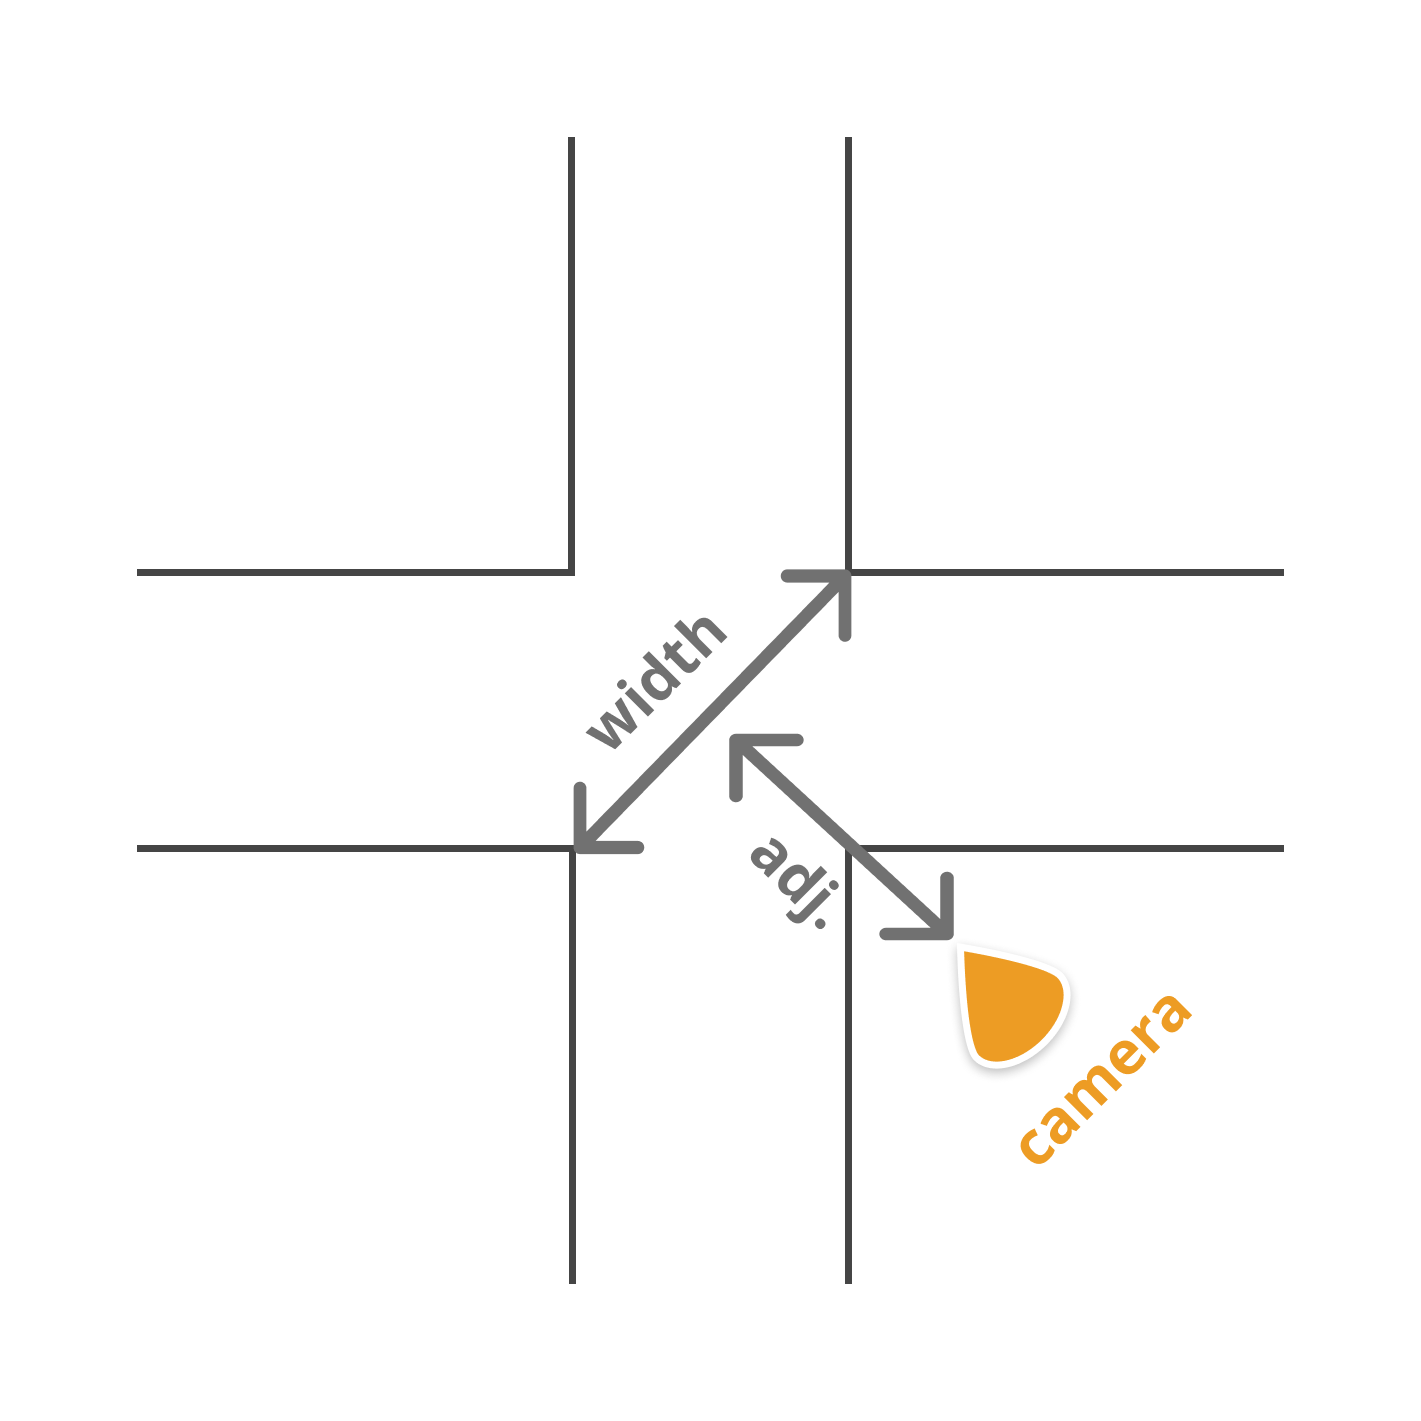
\includegraphics[scale=1.0]{location.png}
    \centering 
    \end{figure}
    \captionof{figure}{Barrel Distortion}
    \label{Camera location}

Battery life should also being considered depending on the amount of intended recording. 149MB per 1 min at 30FPS

\subsection{Data Processing}

\ \\ 
\noindent
\begin{tabular}{@{}cc}
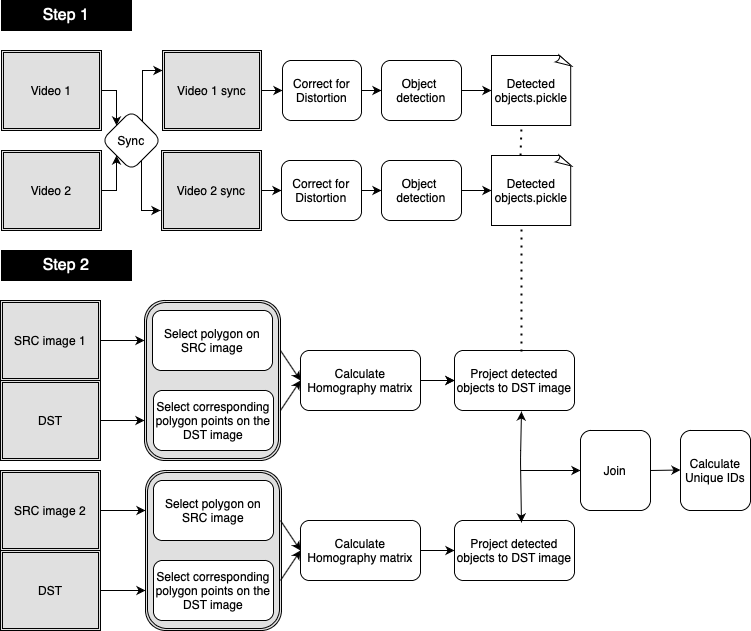
\includegraphics[width=1.0\columnwidth]{data_flow.png} 
\end{tabular}
\captionof{figure}{Data Pipeline}
\label{data}


Figure \ref{data} offers a general overview of the data processing steps. The processing happens on two 
video sources that are cut to the same time period. No special hardware is required, but a CUDA enabled GPU
device would speed up the object detection process.
\ \\
\subsection{Distortion Correction}

Wide angle camera lenses such as that on the LG G6 used in this study produce images that have an optical aberration where straight lines appear bent. 
The specific type being barrel distortion such as in figure \ref{distortion}, where lines curve inwards in a shape of a barrel.

\ \\ 
\begin{figure}[h]
  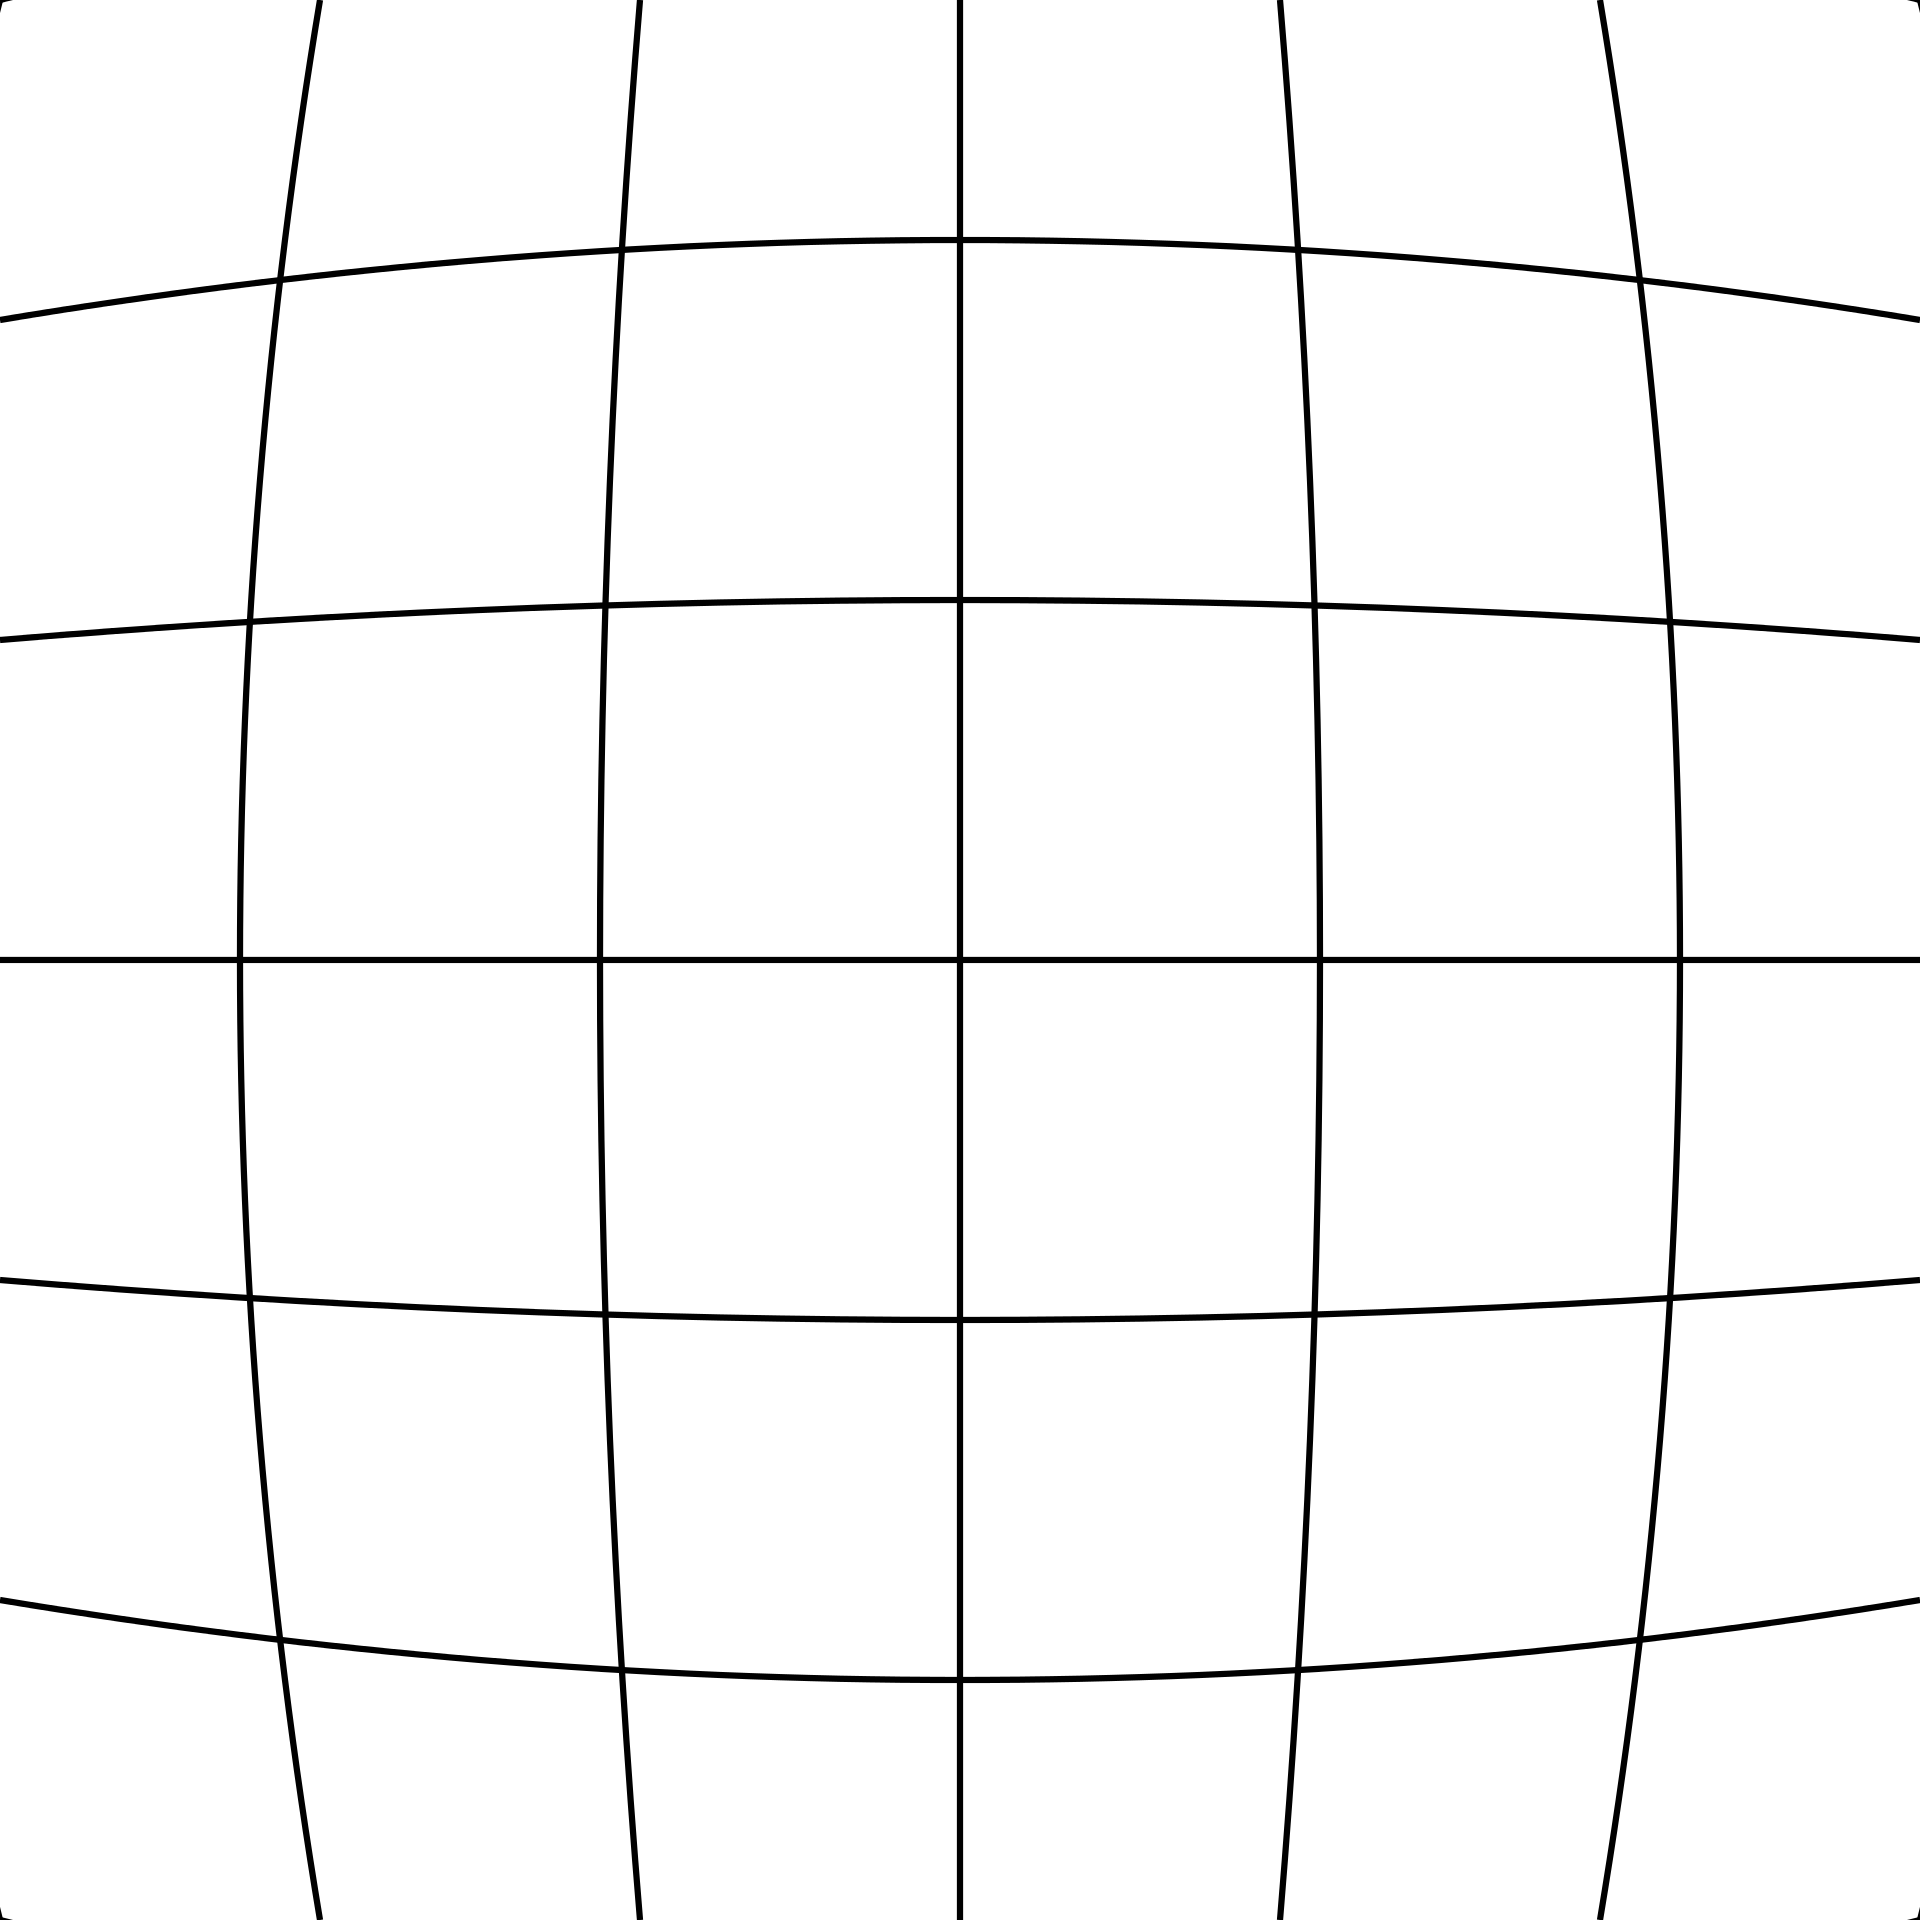
\includegraphics[scale=0.05]{Barrel_distortion.svg.png}
  \centering 
  \end{figure}
  \captionof{figure}{Barrel Distortion}
  \label{distortion}

\ \\
This can lead to incorrect projection and therefore joining of video sources later on.
To correct for this we make use of OpenCVs \cite{noauthor_opencv/opencv_2021} camera calibration toolbox.

Explain this a bit more. Formulas
\ \\
\subsubsection{Object Detection}

The raw video is output as a .mp4 file this video file is if fed to YOLO v5 for object detection. YOLO, You Only Look Once,
is a real-time object detection algorithm. ....Explain more.... 
\ \\ 
Why YOLO v5?
\ \\ 
Objects are detected each frame and represented as bounding boxes.
The output from YOLO is as follows: \[ [frame id][xmin][ymin][xmax][ymax][confidence]  \]

The min and max values for x and y represent a bounding box for the identified bicylce.

Figure \ref{data_pipeline} demonstrates the data pipeline that the output from YOLO is fed through. .
\ \\
\subsubsection{Homography Matrix}

First explain the concept of the homography matrix.
\ \\ 
\begin{figure}[h]
  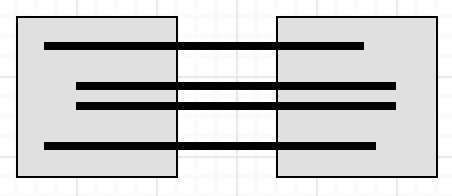
\includegraphics[scale=1.0]{Homography_proj.png}
  \centering 
  \end{figure}
  \captionof{figure}{SR to DST}
  \label{homography}

To transform the data to onto the a new plane view we needed to find the homography matrix, which is a transformation matrix between two planes \cite{hartley_zisserman_2004}.
The homography matrix (H) is a 3×3 matrix with 8 degrees of freedom, this allows the transformation of the cycling objects $P(x_r, y_r)$ to a 
top-down aerial view $P(x_i, y_i)$. The top-down view being an aerial image of the Dybbelobrø intersection and P being the image coordinates in pixel units.

\begin{equation}
  P = HQ\label{eq:2}
\end{equation} 

\begin{align}
\label{eq:3}
  \begin{bmatrix}
    x_{i} \\
    y_{i} \\
    z_{i} \\
  \end{bmatrix}
  &= \begin{bmatrix}
      h_1 & h_2 & h_3 \\
      h_4 & h_5 & h_6 \\
      h_7 & h_8 & h_9 \\
  \end{bmatrix}
  \begin{bmatrix}
    x_{r} \\
    y_{r} \\
    z_{r} \\
  \end{bmatrix}
\end{align}
\subsubsection{Projection}

After finding the homography matrix we can now project to contact points of the bicycle and the road surface onto the destination
image being an aerial view of Dybbelsbrø. This is achieved by applying $z$ to each point as a constant so as to create $Q(x_i, y_i, 1)$ and then we multipy it by 
homography matrix. 
\ \\
\subsubsection{Merging Sources}

To merge the data from the two video sources we take a naive approach. As the cameras are setup on
opposite siders of the intersection for optimal coverage we simply cut the video sources in half along the halfway point between
the two cameras along the intersection. The data is then merged.
\ \\
\subsubsection{Multiple object tracking}

In order to connect observations into trajectories of individual cyclist we apply 
simple online and real time tracking algorithm, SORT \cite{abewley_abewley/sort_2021}, as initially described in \cite{Bewley2016_sort}. 
SORT aims to address the problem of multiple object tracking (MOT) where object across frames needs to be connected. 
Explain more about SORT predict bbox then iou for actualy bbox.

The algorithm returns the bounding boxes along with a unique ID associated with each observation.

Using the bounding boxes we calculate the (x, y) co-ordinates of the observation and shift the y value down onto 
the same plane as the street so as to have the conact point of a bicycles and the street.

\subsection{Data Exploration}

There are two objectives for the data exploration.
\begin{itemize}
	\item1. Rainbow Tracks - Desire path discovery
	\item2. Alert Zones - For behaviour observations and counts
\end{itemize}

\subsubsection{Rainbow Tracks}

\ \\ 
\noindent
\begin{tabular}{@{}cc}
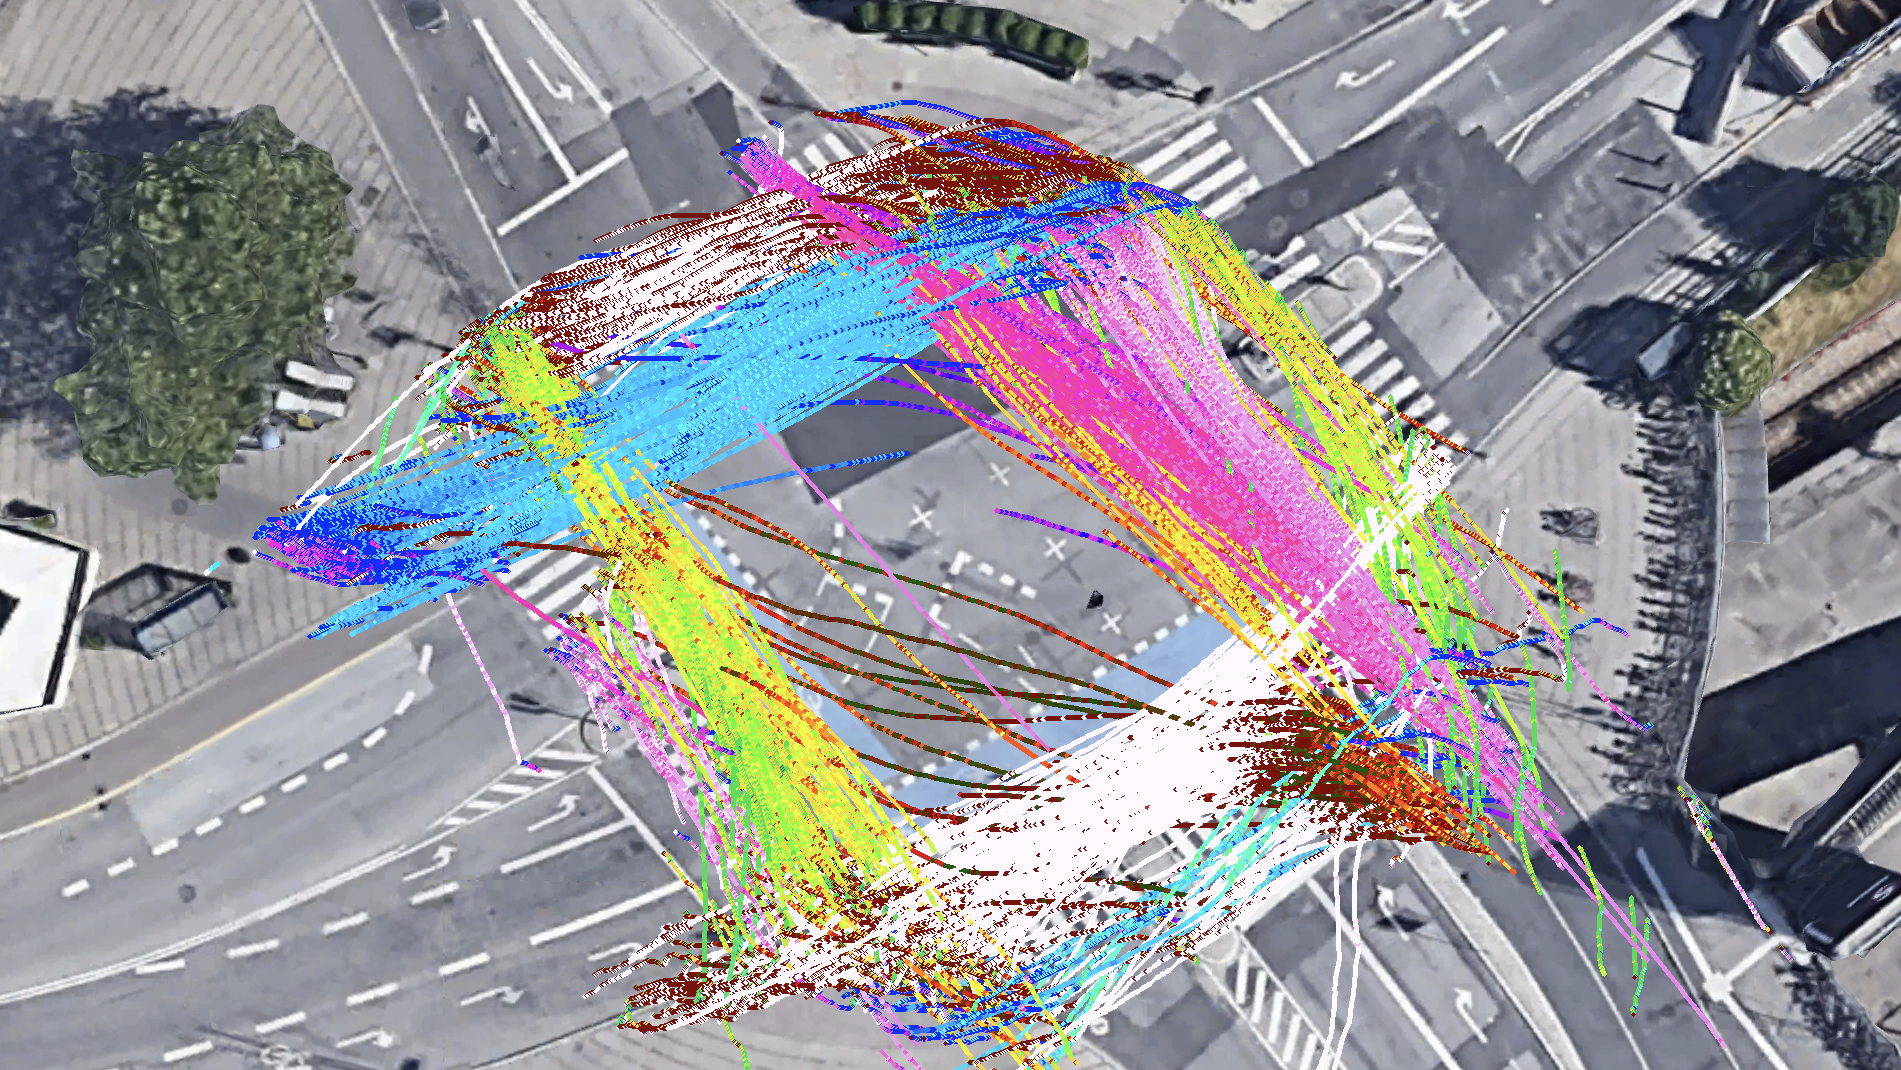
\includegraphics[width=1.0\columnwidth]{rainbow.png} 
\end{tabular}
\captionof{figure}{Rainbow}
\label{Rainbow}

To find aggregated desire lines from the data we took an approach which we call "Rainbow tracks". This involves coloring tracks by the bearing between consequtive points in each 
trajectory, after calculating the bearing we then get a color from a gardient color wheel. This approach has the added benefit of encoding direction into 
each track.
Maybe just an equation demonstaring the bearing calculation.
\ \\ 
\begin{equation}
  UniqueID_i = [(x_1, y_1)...(x_a+1, y_a+1)]\label{eq:3}
\end{equation}

\subsubsection{Alert Zones and Counts}

We created a "Tool name", that allows the defining of certain areas as "Red zones". These zones are provide us with easy reference to activty in the zones throught the videos.
Using these zones we can count cyclist and observe their behaviour at points on the intersection that might be difficult or
problematic.

Picture of interface?
